\
\newpage
\addtocounter{problemctr}{1}
\noindent
{\bf
Problem \theproblemctr.  (\thedfastates \xspace points)}
\swallow{ (\thedfastatestime\xspace minutes)}

\smallskip

\noindent Let $L$ = $b^*a^*$. Please draw a DFA for $L$ below.

\vspace*{6em}
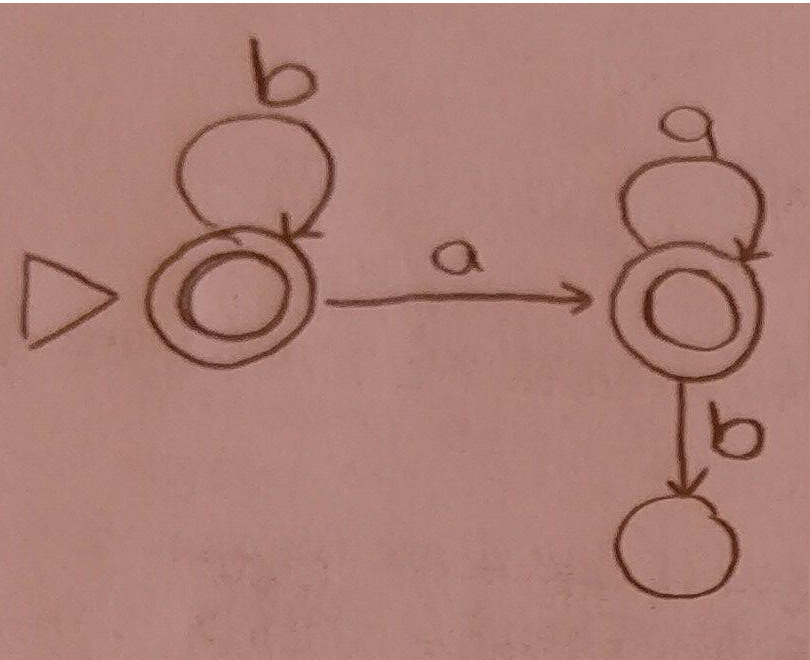
\includegraphics[scale=0.25]{dfa.jpg}
\vspace*{6em}


\noindent How many equivalence classes for $L$ are there?
\rule{1cm}{.01in}3\rule{1cm}{.01in}

\bigskip

\noindent
Please list them below.

\bigskip


\rule{2cm}{.01in}$[b^*],[bb*a],[\Sigma^*a\Sigma^*b\Sigma^*]$\rule{2cm}{.01in}

\bigskip

\noindent Use your findings above to prove that any DFA for L must have at least two
accepting states.


If we assume for sake of contradiction that L has fewer than 2 accepting states:
\begin{itemize}
    \item there can't be 0 accepting states because at least one string (ba) is in the language
    \item If there is 1 state, the for any string accepted by the DFA, the same transition will bring both to the same state. However, 'b' and 'ba' are both in the language and should be part of the same state - appending 'b' to both yields $'bb'\in L$ and $'bab'\not\in L$, a contradiction that proves the assumption false.
\end{itemize}